\documentclass[10pt]{beamer}
\usepackage[T1]{fontenc}
\usefonttheme{professionalfonts}
\usepackage[sfmath,slantedGreeks]{kpfonts}
\usepackage[utf8]{inputenc}
\usepackage[italian]{babel}

\usepackage{booktabs,particlessymb,siunitx}
\usepackage[font=scriptsize,labelformat=empty]{caption}

\DeclareSIUnit\parsec{pc}
\DeclareSIUnit\clight{\text{\ensuremath{c}}}
\sisetup{per-mode=symbol,
  inter-unit-separator={}\cdot{},
  exponent-product=\cdot,
  output-product=\cdot,
  separate-uncertainty=true
}

\renewcommand{\phi}{\varphi}
\renewcommand{\epsilon}{\varepsilon}

\newcommand*{\dd}{\mathop{}\!\textup{d}} % Operatore differenziale \dd
% Derivata totale: \toder[ordine]{funzione}{variabile}
\newcommand*{\toder}[3][]{\frac{{\dd^{#1}}#2}{\dd {#3}^{#1}}}

\title{Raggi cosmici}
\author{Mosè Giordano}
\date{XX aprile 2013}
\institute[UniSalento]{Università del Salento}
\usetheme{Madrid}
\setbeamercovered{dynamic}
\usecolortheme{beaver}
% beaver è un tema grigio-rosso, ma non cambia il colore dei bullet di itemize e
% di enumerate.  Il seguente comando serve impostarli al colore darkred definito
% nel tema beaver.
\setbeamercolor{local structure}{fg=darkred}

\begin{document}
\begin{frame}
  \maketitle
\end{frame}

\begin{frame}
  \frametitle{Piano della presentazione}
  \tableofcontents
\end{frame}

\section[Intro]{Introduzione}

% Per l'introduzione vedi l'articolo arXiv:1302.3307 e
% http://arstechnica.com/science/2013/02/supernova-observations-solve-the-mystery-of-cosmic-ray-origins/
% (questo può essere carino per l'inizio, parla della OMG particle)
\begin{frame}
  \frametitle{}

\end{frame}

\section[Fermi]{Fermi Gamma-ray Space Telescope}

\begin{frame}
  \frametitle{Fermi: l'esperimento}
  \begin{figure}
    \centering
    % Fonte:
    % http://commons.wikimedia.org/wiki/File:Diagram_of_the_GLAST_instrument.jpg
    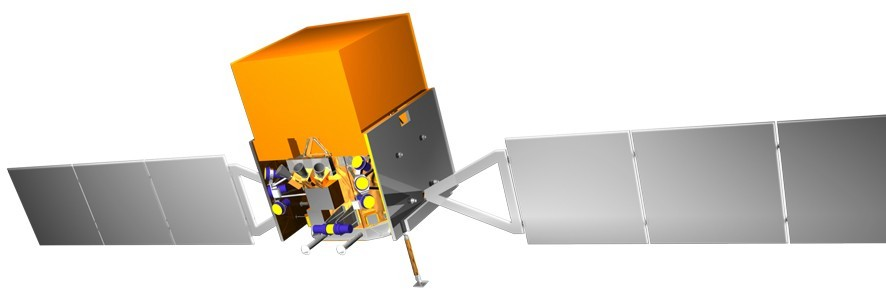
\includegraphics[width=0.5\columnwidth]{glast.jpg}
  \end{figure}
  Osservatorio per lo studio dei raggi gamma (da \SI{8}{\kilo\electronvolt} fino
  a oltre \SI{300}{\giga\electronvolt}) emessi da corpi celesti.  Obiettivi:
  dell'esperimento
  \begin{itemize}
  \item comprensione meccanismo di accelerazione particelle in AGN, pulsar e SNR
  \item studio sorgenti gamma non identificate e radiazione gamma diffusa
    galattica ed extra-galattica
  \item studio emissione ad altissima energia nei GRB
  \item rivelazione indiretta della materia oscura, attraverso suo decadimento o
    annichilazione in fotoni o elettroni e positroni
  \item osservazione evaporazione di MBH dalla presunta traccia di lampi gamma
  \end{itemize}
  È in orbita a \SI{550}{\kilo\metre} d'altezza dall'11 giugno 2008
\end{frame}

\begin{frame}
  \frametitle{Fermi: strumentazione}
  % Per approfondire vedi
  % http://www.nasa.gov/mission_pages/GLAST/spacecraft/index.html
  \begin{columns}
    \begin{column}{0.4\columnwidth}
      \begin{itemize}
      \item Large Area Telescope (LAT), sensibile a singoli raggi gamma con
        energia tra \SI{20}{\mega\electronvolt} e \SI{300}{\giga\electronvolt}
      \item Gamma-Ray Burst Monitor (GBM), studio di fenomeni transienti (GRB e
        brillamenti) a energie relativamente più basse (tra
        \SI{8}{\kilo\electronvolt} e \SI{40}{\mega\electronvolt})
      \end{itemize}
    \end{column}
    \begin{column}{0.6\columnwidth}
      \begin{figure}
        \centering
        % Fonte: http://commons.wikimedia.org/wiki/File:GLAST_schematic.jpg
        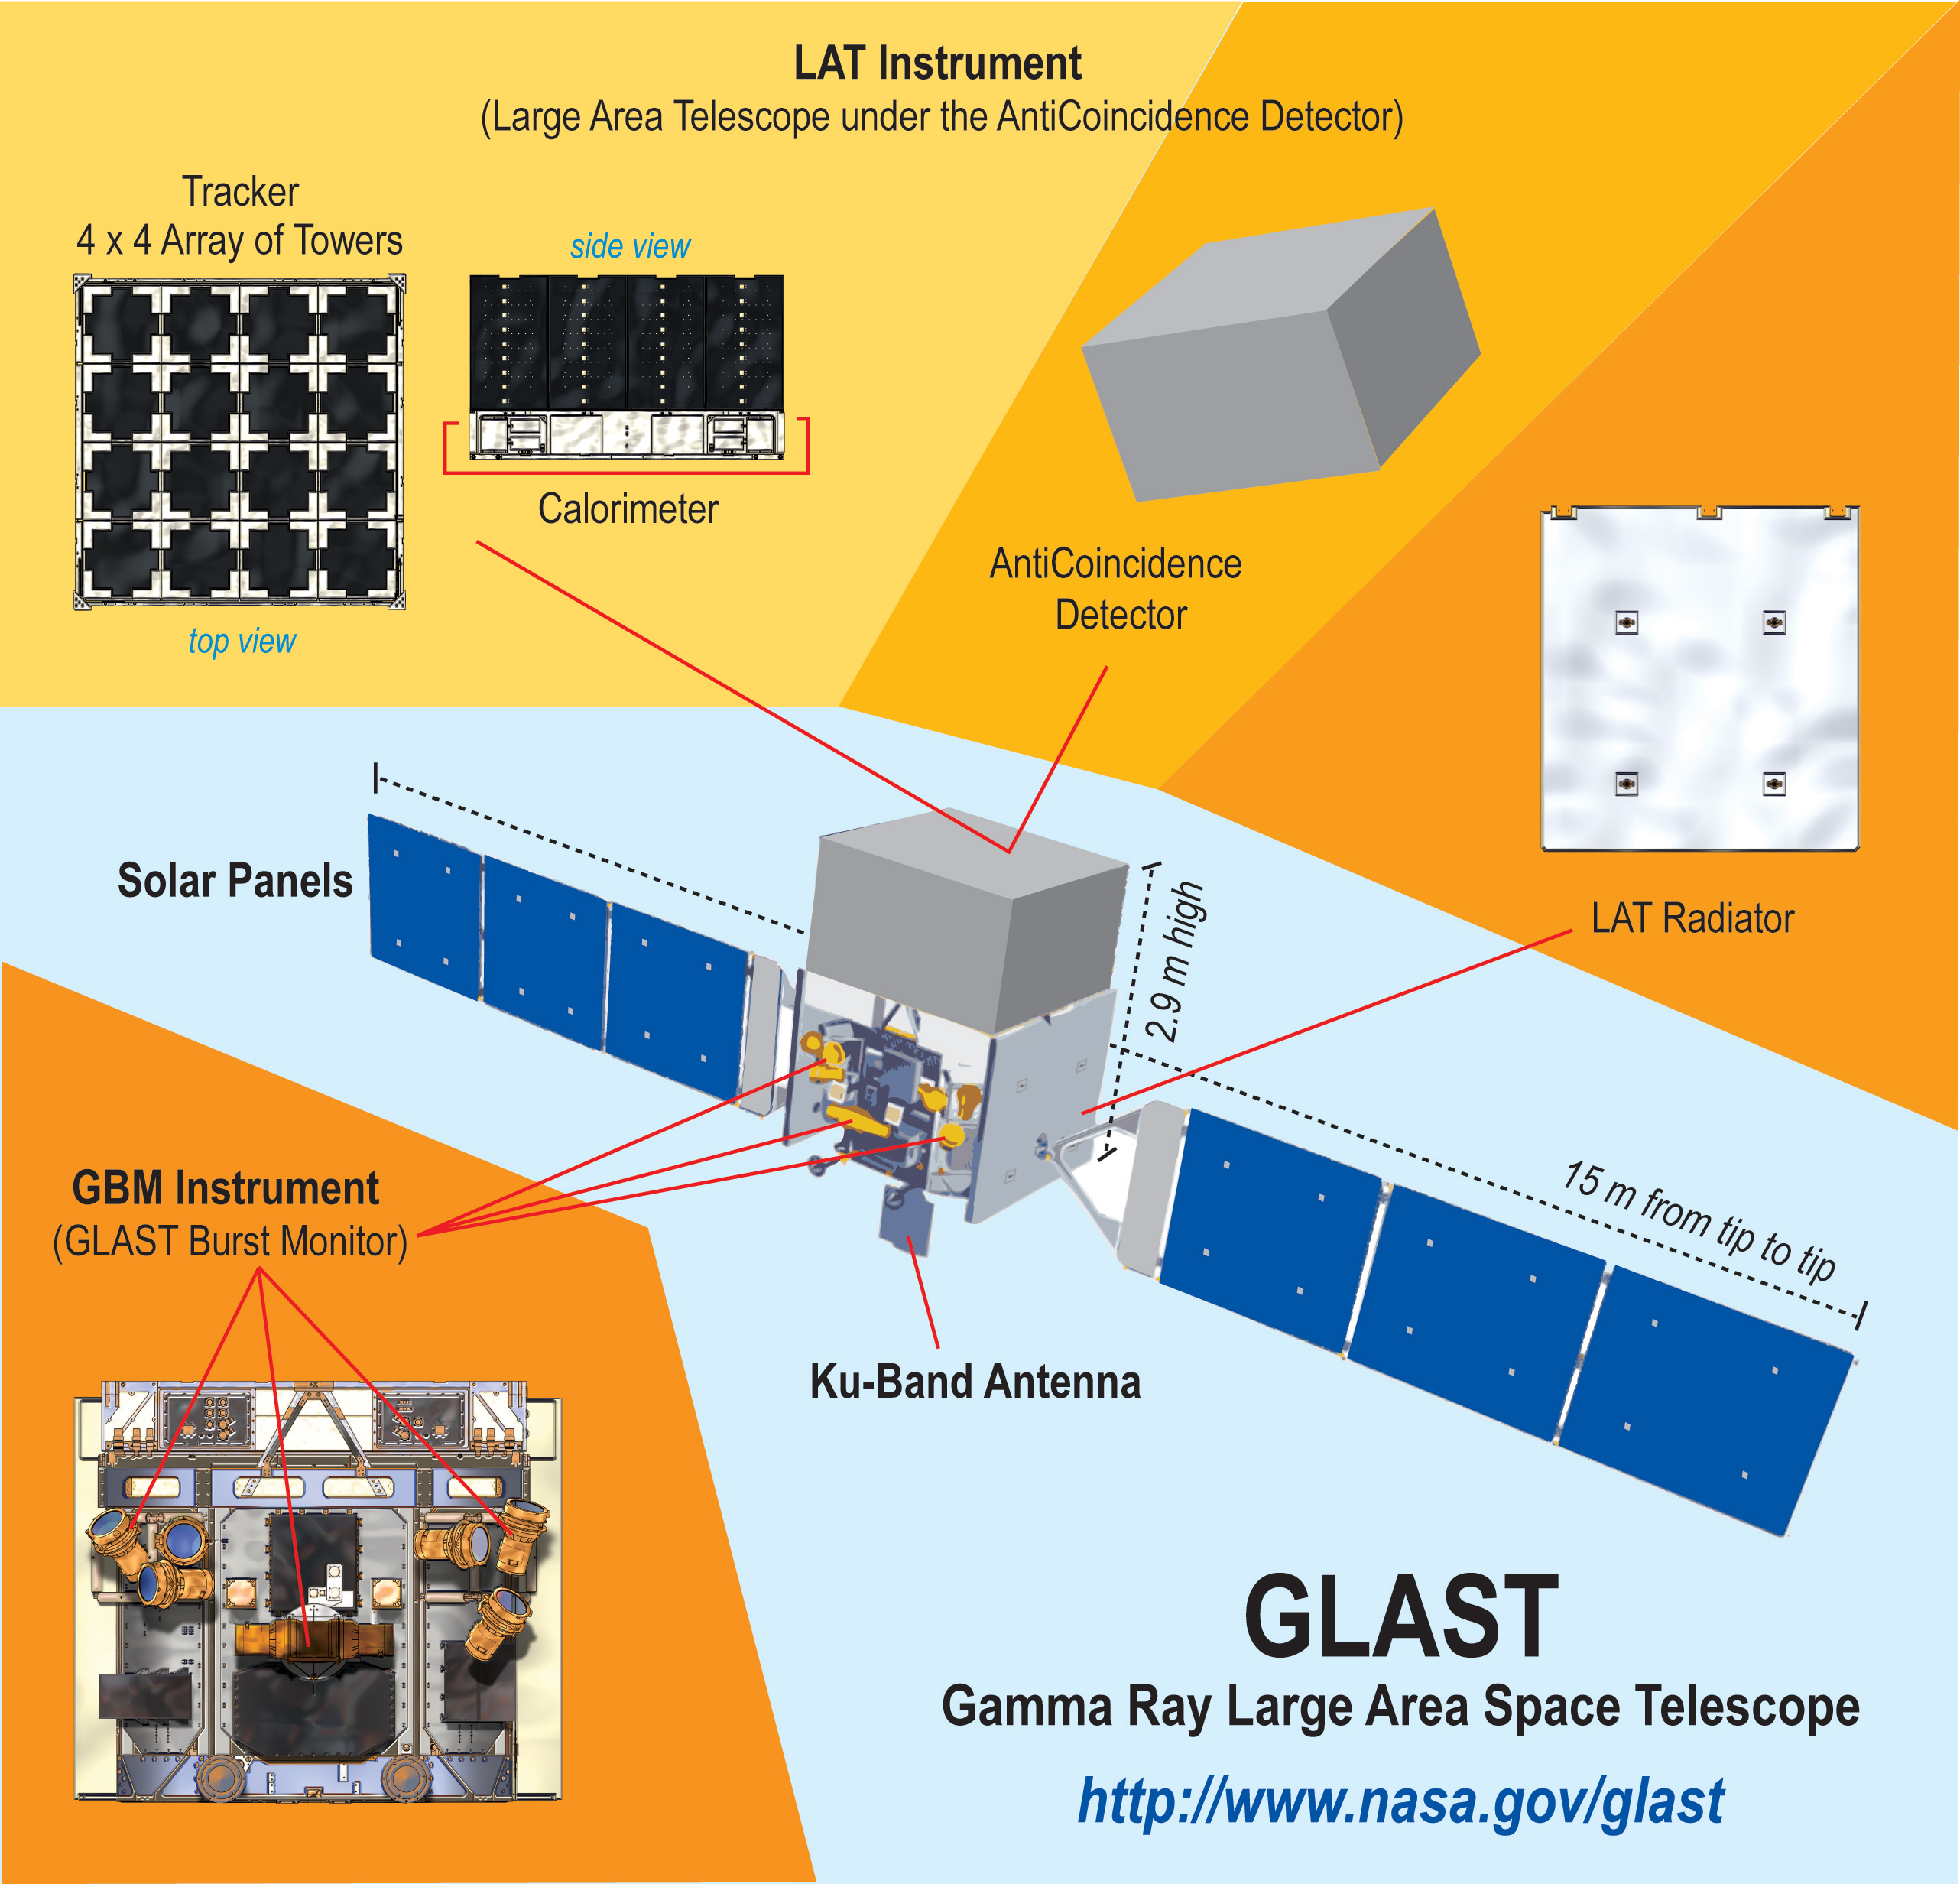
\includegraphics[width=\columnwidth]{glast_schematic.jpg}
      \end{figure}
    \end{column}
  \end{columns}
\end{frame}

\begin{frame}
  \frametitle{Fermi: LAT}
  % Importante: eliminazione del rumore costituito da raggi cosmici, vedi
  % sito indicato sopra.  Vedi anche
  % http://www-glast.stanford.edu/instrument.html
  \begin{figure}
    \centering
    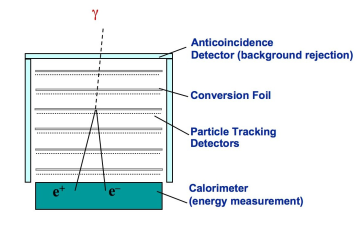
\includegraphics[width=0.6\columnwidth]{Gamma_telescope_schematic}
    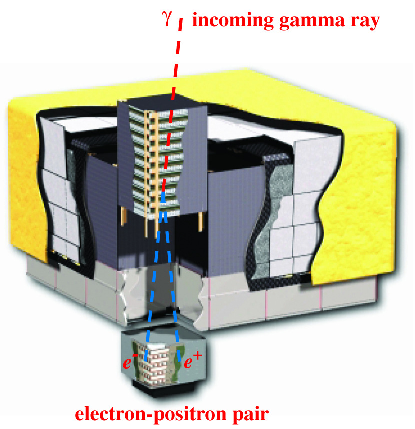
\includegraphics[width=0.4\columnwidth]{f1}
  \end{figure}
\end{frame}

\begin{frame}
  \frametitle{Fermi: SNR osservate}
  \begin{figure}
    \centering
    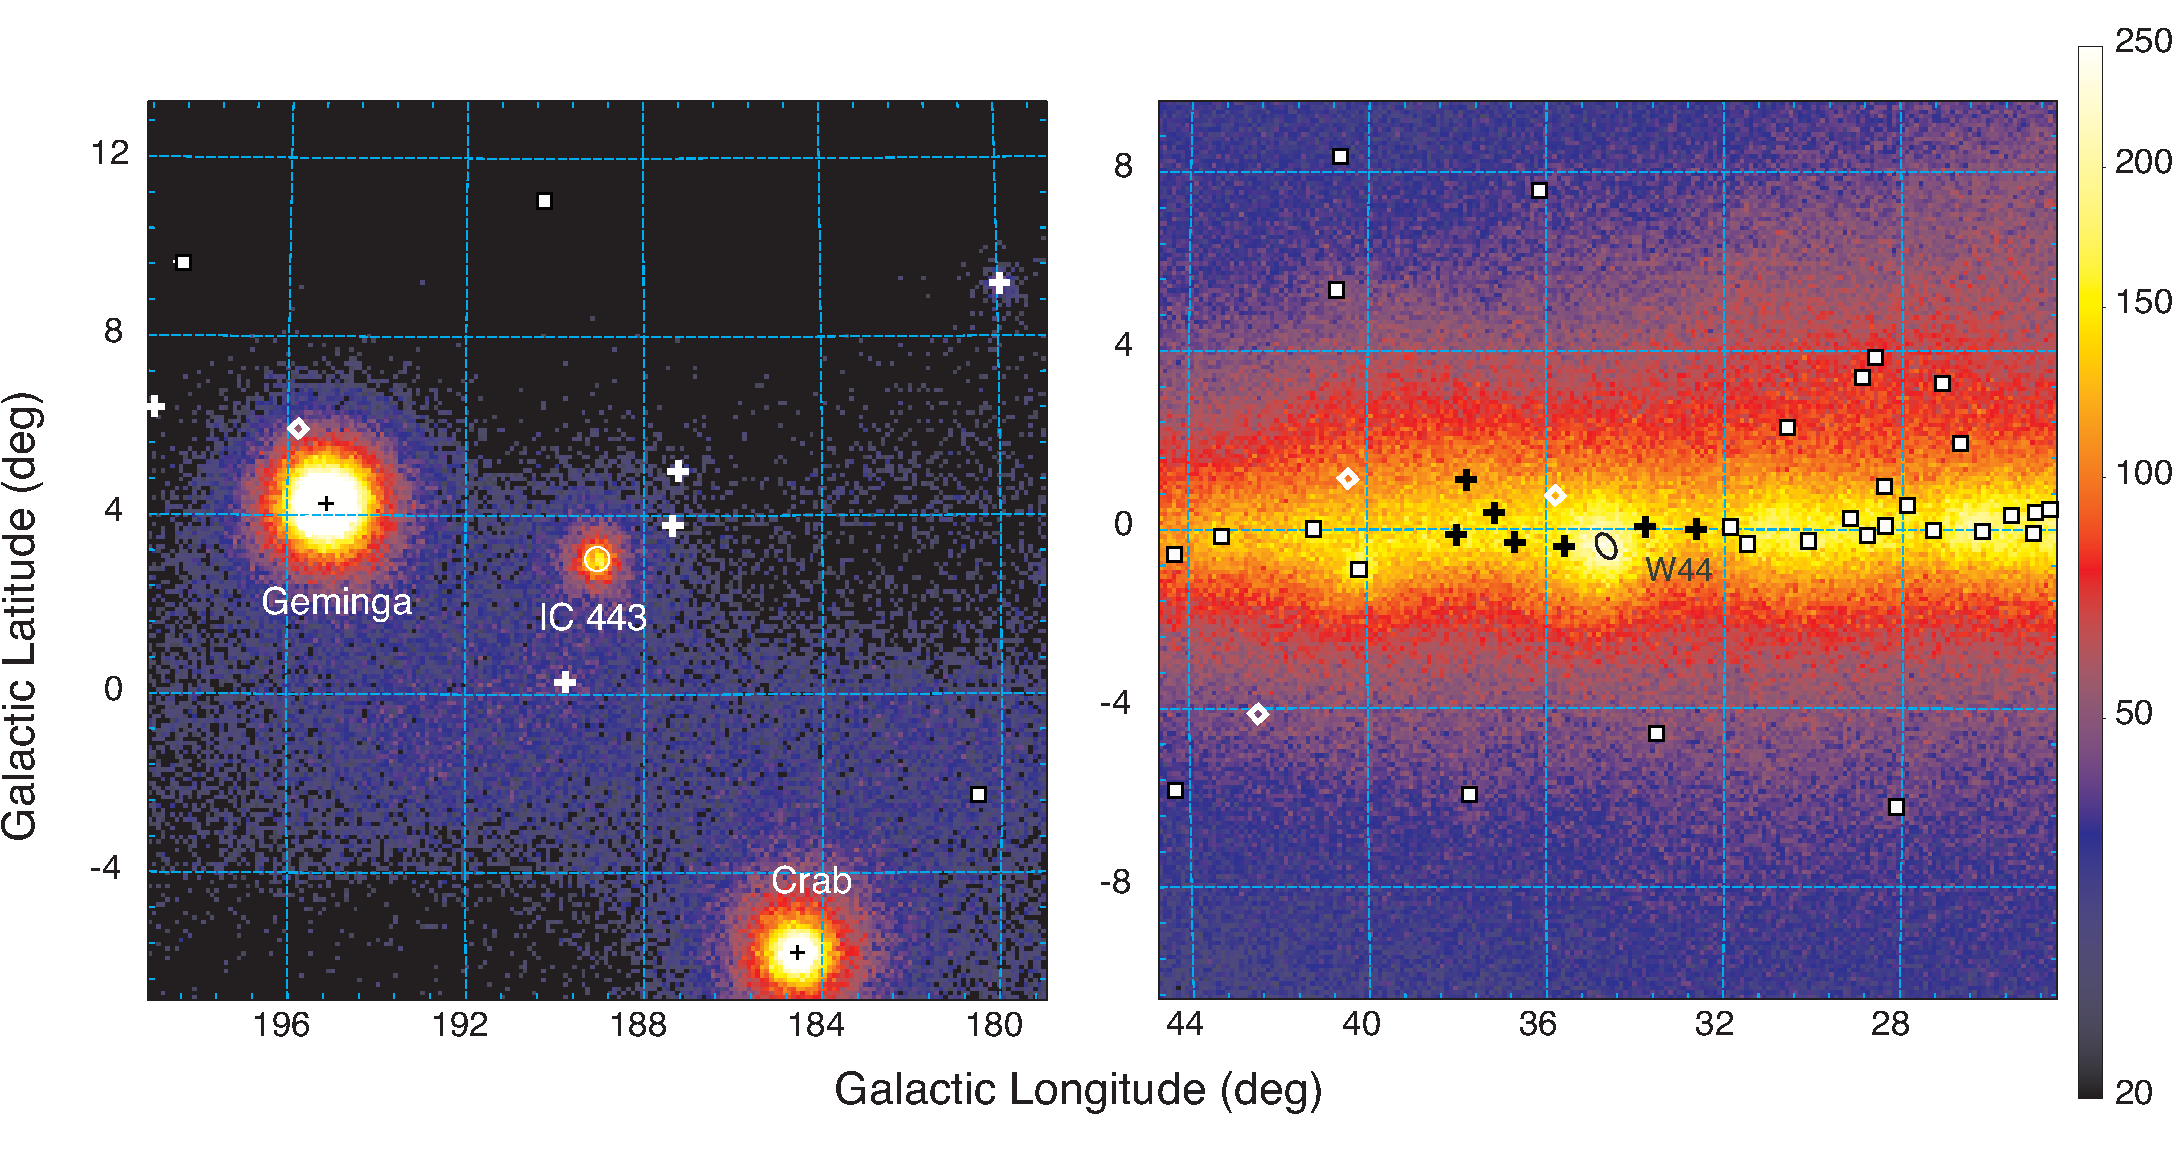
\includegraphics[width=0.8\columnwidth]{1231160fig1.pdf}
    \caption{Mappa del conteggio di raggi gamma in un campo di
      $\SI{20}{\degree} \times \SI{20}{\degree}$ attorno a IC 443 (sinistra,
      \SI{1.5}{\kilo \parsec}) e W44 (destra, \SI{2.9}{\kilo \parsec})
      nell'intervallo di energia da \SI{60}{\mega\electronvolt} a
      \SI{2}{\giga\electronvolt}.  Quadrati e croci indicano sorgenti gamma
      vicine, i rombi sorgenti precedentemente sconosciute.}
  \end{figure}
\end{frame}

\begin{frame}
  \frametitle{Fermi: analisi dei dati}
  \begin{figure}
    \centering
    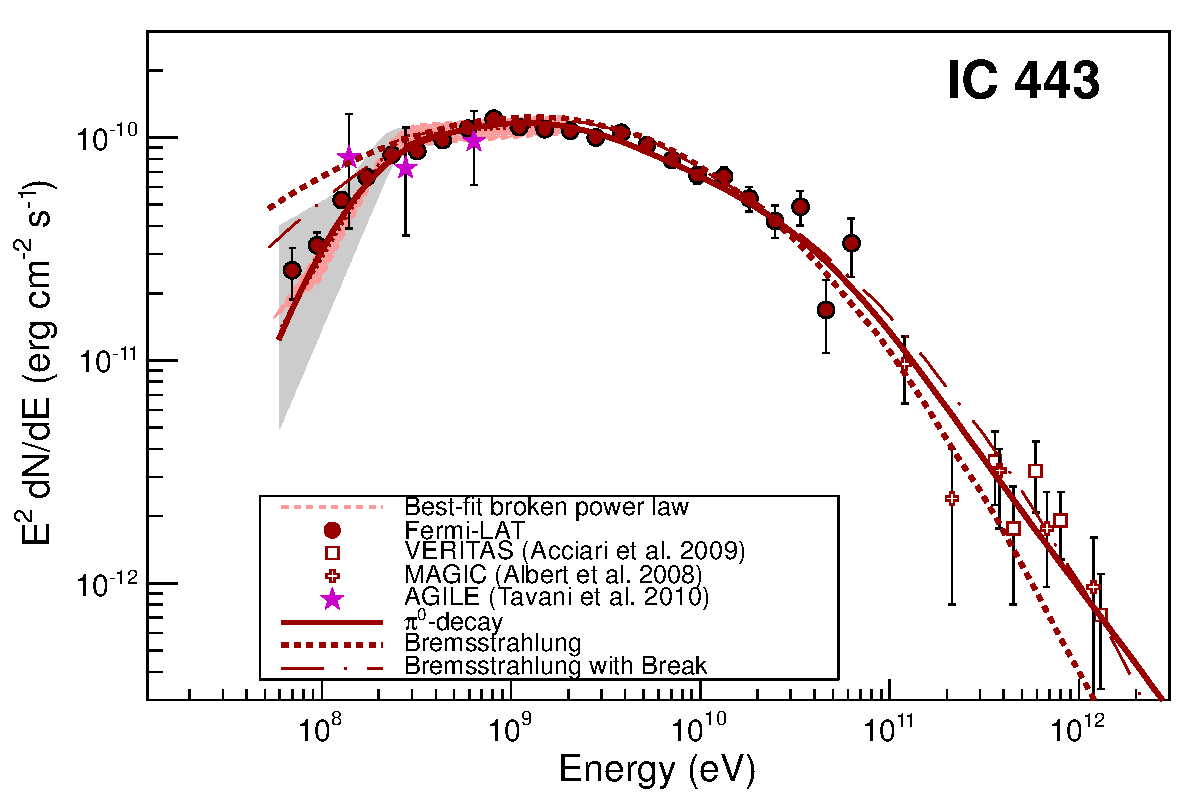
\includegraphics[width=0.5\columnwidth]{1231160fig2a}
    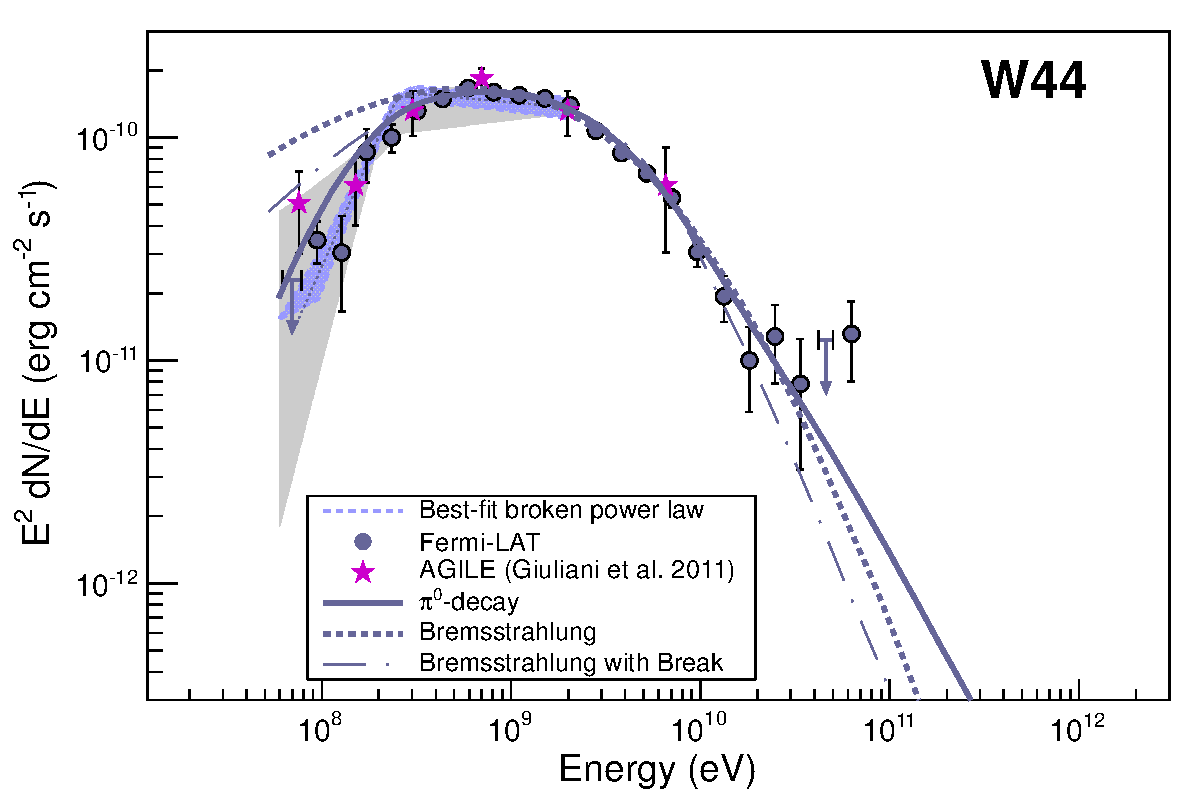
\includegraphics[width=0.5\columnwidth]{1231160fig2b}
    \caption{Spettro dei raggi gamma di IC 433 e W44, misurato da Fermi-LAT}
  \end{figure}
\end{frame}

\begin{frame}
  \frametitle{Fermi: analisi dei dati (cont.)}
  Power law (PL):
  \begin{equation*}
    F(\epsilon) = K
    \left(
      \frac{\epsilon}{\epsilon_{0}}
    \right)^{-\Gamma_{1}}
  \end{equation*}
  Smoothly broken power law (BPL):
  \begin{equation*}
    F(\epsilon) = K
    \left(
      \frac{\epsilon}{\epsilon_{0}}
    \right)^{-\Gamma_{1}}
    \left(
      1 +
      \left(
        \frac{\epsilon}{\epsilon_{\textup{br}}}
      \right)^{(\Gamma_{2} - \Gamma_{1})/\alpha}
    \right)^{-\alpha}
  \end{equation*}
  $\epsilon_{0} = \SI{200}{\mega \electronvolt}$, parametro di smoothness del
  break fissato a $\alpha = 0.1$
  \begin{table}
    \centering
    %\sisetup{per-mode=reciprocal}
    \resizebox{\columnwidth}{!}{\begin{tabular}{cccccc}
        \toprule
        Modello & $K$ (cm\ap{$2$}s\ap{$-1$}MeV\ap{$-1$})
        & $\Gamma_1$ & $\Gamma_2$ & $\varepsilon_{\textup{br}}$
        (\si{\mega \electronvolt}) & $TS$ \\
        \midrule
        IC~443 & & & & & \\
        PL & $11.7 \pm 0.2) \times 10^{-10}$ & $1.76\pm 0.02$
        & $\cdots$ & $\cdots$  &  21651 \\
        BPL & $(11.9 \pm 0.6) \times 10^{-10}$ & $0.57\pm 0.25$
        & $1.95^{+0.02}_{-0.02}$ & $245^{+16}_{-15}$  &  22010\\
        \midrule
        W44 & & & & & \\
        PL & $(13.0 \pm 0.4) \times 10^{-10}$ & $1.71\pm 0.03$
        & $\cdots$ & $\cdots$  &  6920 \\
        BPL & $(15.8 \pm 1.0) \times 10^{-10}$ & $0.07\pm 0.4$
        & $2.08^{+0.03}_{-0.03}$ & $253^{+11}_{-11}$  &  7351 \\
      \bottomrule
    \end{tabular}}
  \end{table}
\end{frame}

\begin{frame}
  \frametitle{Fermi: analisi dei dati (cont.)}
  \begin{figure}
    \centering
    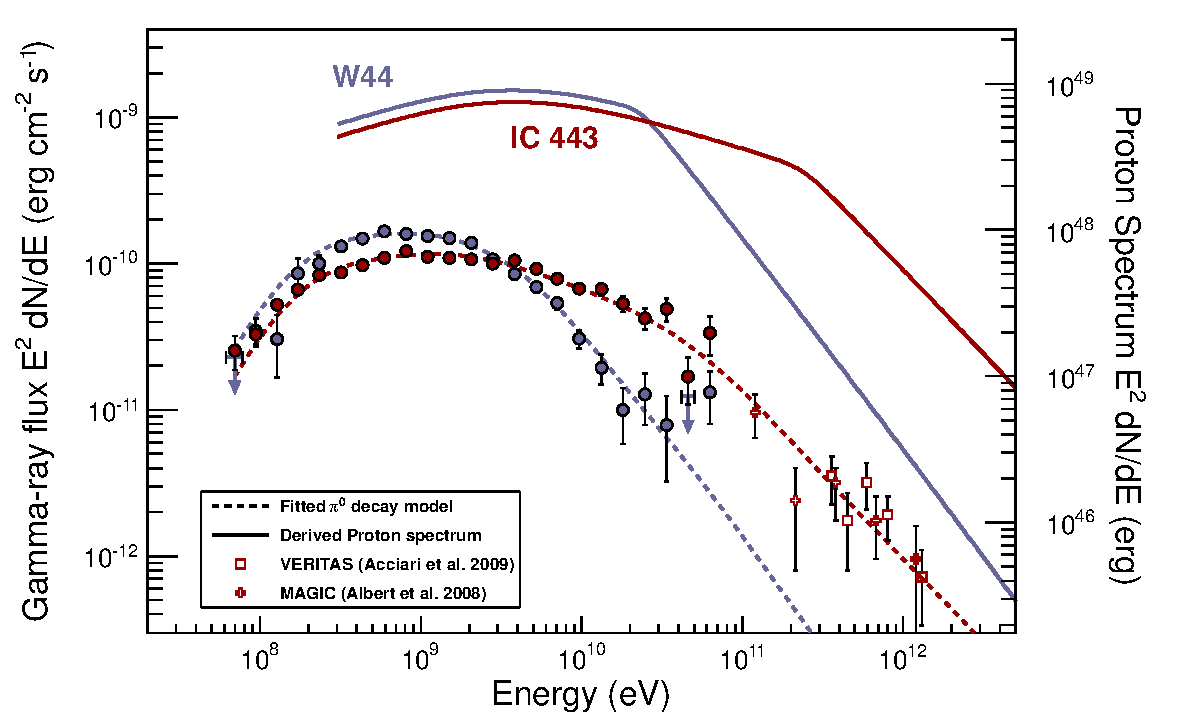
\includegraphics[width=.8\columnwidth]{1231160fig3}
    \caption{Spettro dei raggi gamma e dei protoni progenitori, derivato dallo
      spettro dei raggi gamma.}
  \end{figure}
\end{frame}

\begin{frame}
  \frametitle{Fermi: analisi dei dati (cont.)}
  Lo spettro dei supposti protoni progenitori è stato derivato da una BPL della
  forma
  \begin{equation*}
    \toder{N_{\textup{p}}}{p} \propto
    \left(
      1 +
      \left(
        \frac{p}{p_{\textup{br}}}
      \right)^{(s_{1} - s_{2})/\beta}
    \right)^{-\beta}
  \end{equation*}
  Per IC~443: $s_{1} = \num{2.36(2)}$, $s_{2} = \num{3.1(1)}$,
  $p_{\textup{br}} = \SI{239(74)}{\giga \electronvolt \per \clight}$.  \\
  Per W44: $s_{1} = \num{2.36(5)}$, $s_{2} = \num{3.5(3)}$,
  $p_{\textup{br}} = \SI{22(8)}{\giga \electronvolt \per \clight}$.
\end{frame}

\section[AMS]{Alpha Magnetic Spectrometer}

\begin{frame}
  \frametitle{AMS: l'esperimento}
  \begin{figure}
    \centering
    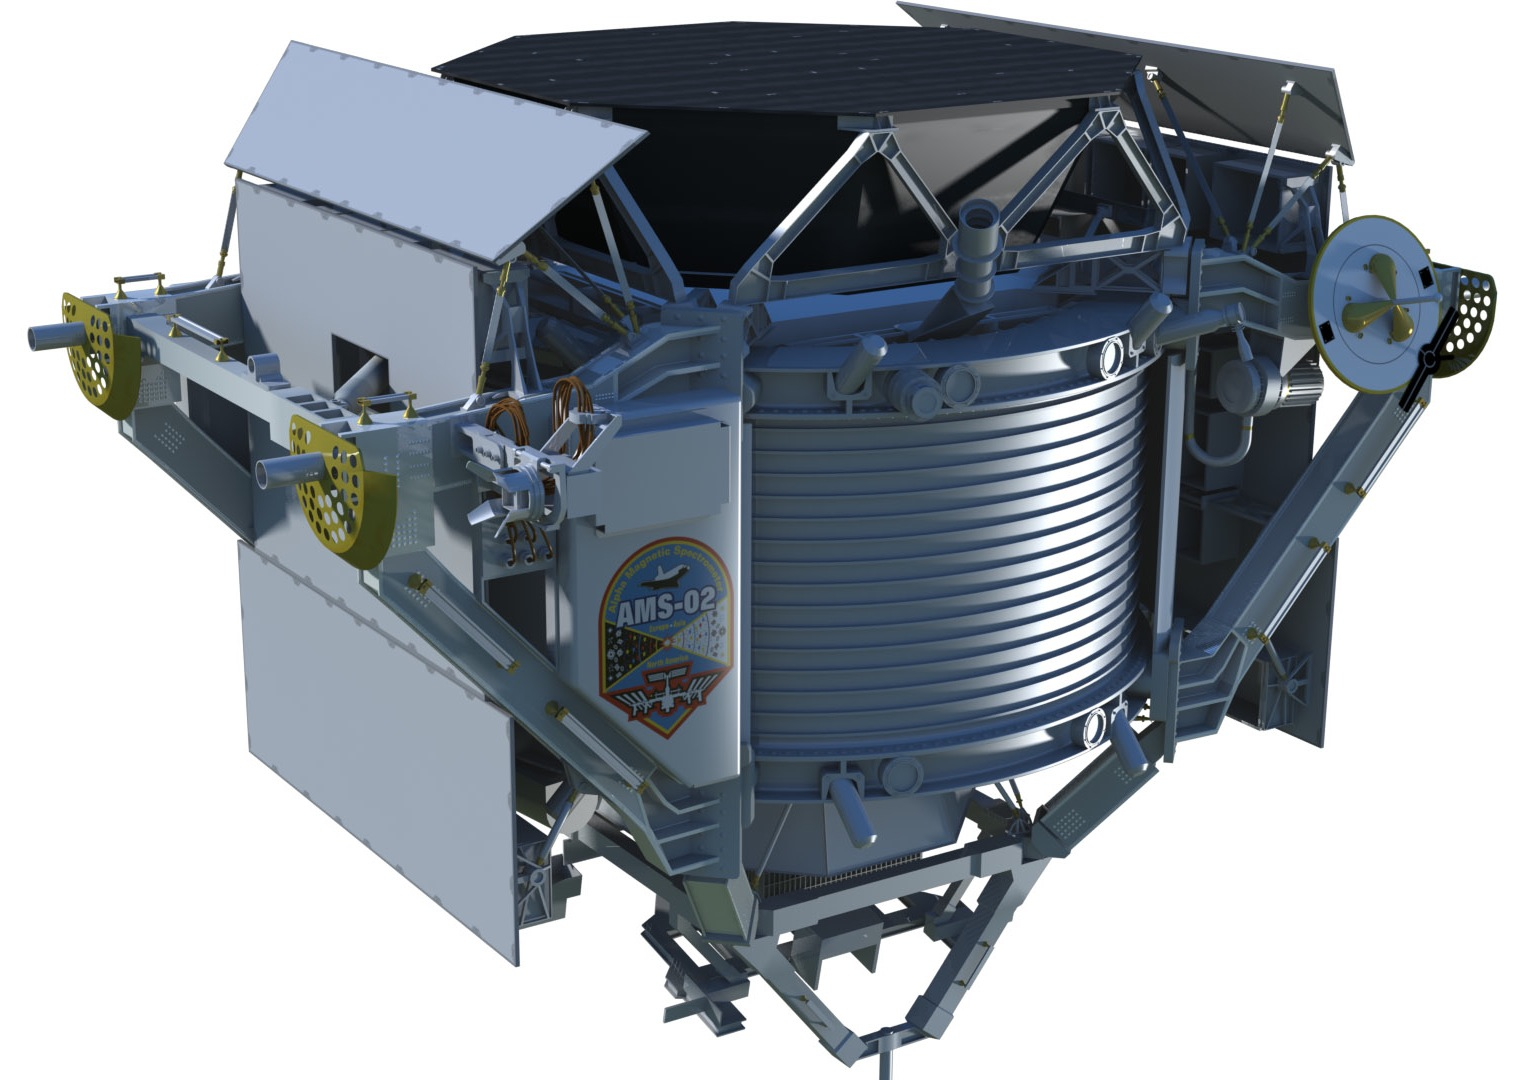
\includegraphics[width=0.3\columnwidth]{ams}
  \end{figure}
  È un modulo per condurre esperimenti di fisica delle particelle ad alte
  energie installato sulla Stazione Spaziale Internazionale.  Obiettivi:
  \begin{itemize}
  \item analisi dei raggi cosmici
  \item studi sulla formazione dell'Universo
  \item ricerca di evidenze di materia oscura
  \item studio dell'antimateria
  \end{itemize}
  È stato montato a bordo della ISS il 19 maggio 2011
\end{frame}
\end{document}

%%% Local Variables:
%%% mode: latex
%%% TeX-master: t
%%% End:
